\section{Versuchsaufbau und Messgeräte}
\subsection{AC-Suzeptibilität}
Die AC-Suzeptibilität ist eine komplexwertige Größe, mit der magnetische Proben gut und recht einfach untersucht werden können. Sie zeigt das Verhalten der Probe in magnetischen Wechselfeldern und kann sehr gut für den Phasenübergang zwischen supraleitender Phase und normalleitender Phase veranschaulicht werden. Bringt man eine leitende Probe in ein magnetisches Wechselfeld, werden in ihre Wirbelströme induziert, welche wiederum ein kleines inneres Magnetfeld verursachen, welches zum ursprünglichen Feld phasenverschoben auftritt. Aufgrund der Wirkung von somit zwei Feldern, treten auch in der Magnetisierung der Probe verschiedene Komponenten auf, welche man allerdings in der AC-Suszeptibilität zusammenfasst:

\begin{align}
\overrightarrow{M}=\left(\chi' - i\chi ''\right)\cdot \overrightarrow{H}=\chi_ac \cdot \overrightarrow{H}
\end{align}

Für die Messung der AC-Suszeptibilität verwenden wir eine spezielle Schaltung, die sogenannte Hartshorn-Spulensystem. Dieses besteht aus einer Primärspule mit 2116 Windungen, welche von einem Wechselstrom durchflossen wird. Das von ihr erzeugte Magnetfeld induziert in zwei Sekundärspulen mit der gleichen Windungszahl wiederum einen Strom, welcher sich aufgrund des entgegengesetzten Windungssinns im nachgeschalteten OPV und Spannungsmessgerät aufhebt. Der Aufbau ist in Abbildung \ref{aufbau-AC} nochmals dargestellt. Bringt man nun in eine der beiden Spulen ein magnetisches Material, ändert sich die Flussdichte in der entsprechenden Spulen und das Messsignal ist ungleich null, welches von der Änderung der Magnetisierung mit dem Magnetfeld H, also von $\frac{\partial M}{\partial H}$ abhängt. Über einen Lock-In-Verstärker wird dabei ein Referenzsignal mit genau bekannter Frequenz in die Primärspule eingespeist. Durch Überlagerung des Ausgangssignals mit dem Referenzsignal lassen sich Störsignale sehr gut herausfiltern, wodurch nur das wirklich vom Referenzsignal erzeugte Ausgangssignal mit exakt der richtigen Frequenz dargestellt werden kann. Über den Lock-In-Verstärker kann weiterhin die Phasenverschiebung zwischen Referenz- und Ausgangssignal gemessen werden. Dabei werden auf das Referenzsignal gezielt verschiedene Phasenverschiebungen geschaltet und das resultierende Überlagerungssignal aus Referenzsignal und Ausgangssignal überprüft. So können verschiedene Phasenverschiebungen eingestellt und gemessen werden. Mit dieser Methode können verschiedenphasige Anteile des Ausgangssignals einzeln gemessen werden. Dies ist sehr wichtig für die Messung der AC-Suszeptibilität, da diese einen mit dem angelegten Feld gleichphasigen Anteil, wie auch einen um $-\frac{\pi}{2}$$ verschobenen Anteil aufweist. 


\begin{figure}[h!]
	\centering
	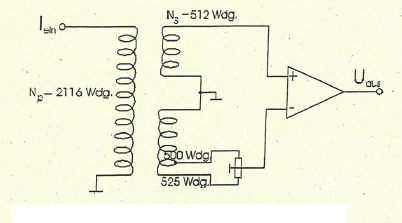
\includegraphics[height=8cm]{AC-auf.png}	
	~ %
	\caption{Hartshorn-Spulensystem für Messung der AC-Suszeptibilität \cite{Anleitung}}
	\label{aufbau-AC}
\end{figure}

\subsection{Phasenübergang der Indiumprobe}
Die Probe befindet sich auf einer Messapparatur in einem aufwändigen Kryostat mit fünf Glasschichten, die von außen nach Innen trennen: Luft ($T=300$K), Vakuum (thermische Isolation), Stickstoff ($T=75$K), Vakuum, Helium ($T=4,2$K), vgl. hierzu Abbildung \ref{aufbau}.

\begin{figure}[h!]
	\centering
	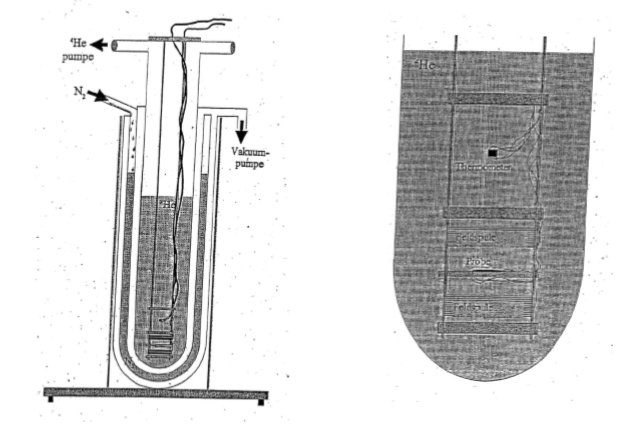
\includegraphics[height=8cm]{Aufbau.png}	
	~ %
	\caption{Messaufbau Phasenübergang Indium-Probe. \cite{Anleitung}}
	\label{aufbau}
\end{figure}

Für Indium gilt erfahrungsgemäß etwa $T_c=3,41$K, was sich unterhalb der Siedetemperatur von Helium befindet. Durch Reduktion des Drucks im Behälter sinkt auch die Siedetemperatur (vgl. Dampfdruckkurve), sodass wir auch Temperaturen unterhalb des klassischen Siedepunkts von Helium erreichen können. So ist es möglich, durch bloßes Öffnen und Schließen der Ventile den Temperaturbereich von $T$=2 bis $T$=4K zu durchfahren. Die Messung des Widerstands geschieht dabei über eine sog. 4-Punkt-Messung, bei der die Probe über vier Messpunkte kontaktiert wird. Dabei wird über zwei Spitzen eine Wechselspannung angelegt, während die anderen beiden Spitzen zur Messung des Spannungsabfalls in der Probe verwendet werden. Diese Methode bietet eine sehr hohe Messgenauigkeit, da die Messleitungen selbst keinen Strom tragen. Über den Lock-In-Verstärker mit gespeicherter Eichkurve werden dabei ständig Messwerte aufgenommen und direkt in ein R-T-Diagramm aufgetragen. Der Lock-In-Verstärker stellt dabei einen sehr engen Bandpassfilter dar, welcher mittels eines Referenzsignals speziell nach der angelegten Frequenz sucht und damit Störsignale quasi ausschließt. Da der Widerstand der Probe in der supraleitenden Phase sehr gering ist, ist eine solche Methode zur Widerstandsmessung unabdingbar. Der Prozess geschieht weiterhin hinreichend langsam, als dass das System im ständigen Gleichgewicht betrachtet werden kann.
